
\part{Un chatbot}

Le but initial d'un chatbot est un agent pouvant dialoguer avec un utilisateur dans un certain contexte, un contexte est un ensemble de mots donnant lieu à un langage.\linebreak
Un modèle très basique de chatbot est un simple programme qui récupère clavier de l'utilisateur puis affiche une réponse formaté, les chatbot basique sont pas aussi intelligents, le contexte de la conversation a besoin d'être conservé pour pouvoir donner un meilleur sens et une interaction bien plus intéressante avec l'utilisateur.\linebreak
\\
Pour qu'un chatbot soit intéressant, celui-ci doit savoir de quoi on parle et savoir donner des réponses pertinentes, sans compter sur la qualité des réponses qui doivent être humainement compréhensible.\linebreak
\linebreak
Dans cette partie, nous allons voir les technologies utilisées, les algorithmes utilisés, des papiers théoriques et pratiques des recherches sur certains algorithmes utilisés et l'assemblage de tous ses composant pour aboutir à un prototype du projet final.

\chapter{Le langage naturel}

Le langage naturel n'est pas aussi facile à interpréter qu'une série de valeurs pour les algorithmes de machine learning, c'est pour cela que pour gérer le langage naturel, nous avons d'autres algorithmes que ceux cité ci dessus.
Nous parlerons de \textit{Sequence To Sequence}, \textit{Long Short Term Memory},  \textit{Conditional Random Field}, \textit{Named Entities Recognition} ou de réseaux bayésiens naïf.\\

\pagebreak
\section{Les réseaux bayésiens naif}

C'est la première référence que nous avons quand on cherche dans le registre du travail avec les chaînes textuelles.\\
L'idée du réseau bayésiens naïf est de représenter un ensemble de documents en une liste de fréquences de pairs $(w, |w|)$, w était un mot dans le langage des documents concernés, pour chaque labels, nous allons construire un modèle de probabilité via la formule suivante:
\formula{$P(X|Y=y)$}
Pour classifier un document, nous allons utiliser la formule ci-dessous et retirer le meilleur résultat en tant que prédiction:
\formula{$ pred = P(X|y) * P(y)$}

D'après le module \textit{Scikit-Learn}, la variante Multinomial se démarque des autres variantes pour des raisons de fonctionnement, la où les autres variantes demandent des cardinaux des mots, le multinomial fonctionne avec l'algorithme nommé \textit{TF-IDF}, cette algorithme sera introduit sous peu.\linebreak
\linebreak
Prenons ses deux corpus suivants, extrait de wikipedia. (le label de chaque corpus est représenté par un mot en gras):\\
\begin{description}
\item[Pomme]: La pomme est un fruit comestible à pépins d'un goût sucré et acidulé et à la propriété la plus ou moins astringente, selon les variétés. D'un point de vue botanique, il s'agit d'un faux-fruit. Elle est produite par les pommiers.
\item[Automobile]: Le terme populaire automobile désigne un véhicule à roues mû par un moteur et destiné au transport terrestre de personnes et de biens.
\end{description}

\pagebreak

La procédure d'apprentissage par Multinomial demande deux traitements sur la donnée, la première est nommée $Tokenization$ et la seconde $Frequencies$:\\
\begin{description}
\item[$Tokenization$]: Pour une chaine textuelle, nous allons supprimer tous les mots $stopwords$ comme $'le','la','ces',...$ des mots qui n'ont aucun impacte sur le sens général du texte, si on applique à $\textbf{Automobile}$ ceci donnerai: 
\begin{description}
\item[] terme populaire automobile désigne véhicule roues moteur destiné transport terrestre personnes.
\end{description}

\item[$Frequencies$]: Pour tous les mots présent dans le texte courant, nous allons lui associer un dans son vecteur, la valeur vide étant zero. Pour que le tableau ne soit pas très large, nous allons prendre ces deux textes suivant: 
\begin{description}
\item[1:] gare train gauche gauche magasin
\item[2:] chaussures rangé haut magasin
\end{description}
Ce qui donne:\\\\
\begin{tabular}{c|c|c|c|c|c|c|c}
$-$ & chaussures & gare & gauche & haut & magasin & rangé & train\\
\hline
1: & 0 & 1 & 2 & 0 & 1 & 0 & 1\\
2: & 1 & 0 & 0 & 1 & 1 & 1 & 0\\
\end{tabular}
\end{description}

\ \linebreak
Pour avoir une implémentation complète venant de $scikit-learn$, la $tokenization$ sera décrit par l'algorithme $CountVectorizer$ et la $Frequencies$ par $TF-idf$.\\
\pagebreak

\section{Conditional Random Field}
Un autre modèle statistique, mais qui cette fois ne s'arrête pas à un simple encodage des variables, mais à de l'extraction de sous chaînes, mais prend aussi en compte les variables voisines, pour correctement illustrer, prenons trois mots d'une phrase, comme $"pour$ $correctement$ $illustrer"$, et prenons le mot $"correctement"$, ce mot sera inséré dans une structure de données ayant comme champs:
\begin{description}
\item[lower]: le mot en minuscule (donc $"correctement"$)
\item[digit]: un boolean disant si le mot est un nombre ou pas
\item[title]: si ce mot est un titre (sous la forme capitalisée)
\item[trois champs -1]: qui lui contient les trois champs du dessus, mais avec le mot $n-1$ 
\item[trois champs +1]: qui lui contient les trois champs du dessus, mais avec le mot $n+1$ 
\end{description}

Ce modèle largement utilisé lorsque qu'on veut traiter le langage naturel donne d'assez bon résultats.\\
\linebreak
Pour appuyer la qualité des résultats, en 2018, l'entreprise Google a développé un algorithme nommé \textbf{BERT} un outil de pré traitement du langage naturel qui a significativement amélioré les algorithmes de traitement du langage naturel. Dans le cadre du CRF nous utilisons le mot $n+/-1$ pour $n$, la où \textbf{BERT} prend en compte aussi les mots $n+/-2$, mais ce n'est pas tout, quand l'algorithme devait être testé, celui-ci devait deviner un mot en index $n$ de la phrase en ayant que ses quatre mots, les résultats étaient correct sans plus, donc en amélioration ils ont finalement laissé le pouvoir à l'algorithme de pouvoir lire la phrase en entier du sens normal (de gauche à droite) et aussi de lire la phrase de droits à gauche, ainsi de considérablement augmenter la précision des réponses.

\pagebreak
\section{Named Entities Recognition}
Dans la catégorie de l'extraction de données, l'extraction des entités nommées consistent à extraire un groupe de mots pouvant décrire des mots clef de type Entreprise, Localisation comme des villes ou des noms...\\
Un exemple de base serait:\\

\formula{la firme Mafirme était présent le mois dernier à Paris pour tenter de gagner 100 000 euros.}

\begin{tabular}{c|cc|c}
Mot & index début & index fin & catégorie \\
\hline
Mafirme & 9 & 15 & Entreprise\\
Paris & 49 & 54 & Localisation\\
100 000 euros & 78 & 91 & Argent\\
\end{tabular}

\ \linebreak
En important un modèle personnalisé notre NER pourrait avoir d'autres utilités, comme par exemple,  nous voulons que notre bot sache répondre dès qu'il  a compris le problème, nous utilisons un NER personnalisé avec une cinquantaine d'exemples afin que notre modèle sache répondre correctement, il bot sait extraire le sujet d'une phrase, par exemple:

\begin{description}
\item[Client]: Depuis cinq jours le tuyau de mon évier de salle de bain fuit à grosse goutte
\item[Bot]: tuyau de mon évier de salle de bain fuit
\end{description}

\pagebreak
\section{Long Short Terme memory}
Commençons les gros algorithmes avec le LSTM, il fait partie de la famille des \textit{Recurrent Neural Network (RNN)}. Les réseaux de neurones récurrents peut être vu comme des combinaisons de circuits imprimés (comme des nos ordinateurs) relié ensemble par de petits ponts de transferts de données. 
Un circuit est représenté par cette illustration suivante:

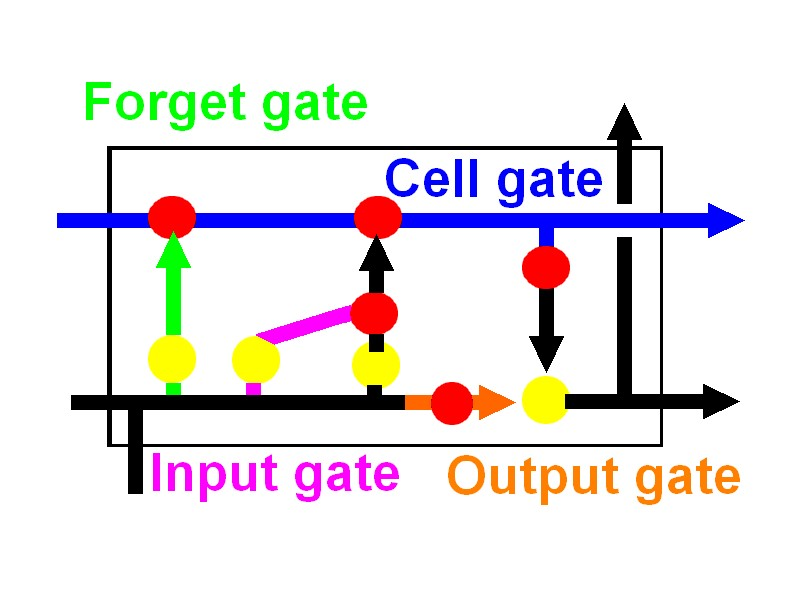
\includegraphics[scale=0.4]{img/lstm.jpg} 

\begin{description}
\item[Forget Gate]: Prenant en entrée le mot à l'indice $N$ et l'information du circuit $N-1$, 
la fonction sigmoid va décider si le circuit va oublier ou garder le mot courant. 
\item[Input Gate]: Ce bout de circuit fait appel aux fonctions sigmoid et tangente, le produit des résultats va déterminer l'importance du mot courant.
\item[Cell State]: Cette partie du circuit va calculer la variable de sortie du circuit.
\item[Output Gate]: Cette dernière partie du circuit va calculer pour le circuit suivant si le prochain mot doit être conservé ou oublier par rapport au résultat donné tout au long du circuit courant.
\end{description}
\ \linebreak

LSTM est comme Seq2Seq, dans son fonctionnement général ils sont égaux, mais LSTM peut couvrir plus de choses que Seq2Seq qui lui a plus une utilité FAQ (pour les Foires Aux Questions il est très adapté) tandis que LSTM peut vraiment tout couvrir, le seul défaut c'est qu'il demande énormément de données, il a un temps d'apprentissage énorme et demande des cœurs GPU (carte graphiques) pour un gain de vitesse considérable.\\
\pagebreak

\section{Sequence To Sequence}
Le modèle Seq2Seq est très puissant, sa structure est donnée par deux colonnes, la première étant n'importe quoi de type texte et la sortie étant aussi n'importe quoi de type texte. Les exemples simples donnés sur le net sont un traducteur anglais vers français ou un générateur de réponses à des questions.\\
\linebreak
Ce processus demande de connaitre à l'avance tous les caractères utilisées pour ainsi transformer chacune des lettres en indice numérique unique, tous les mots seront ensuite remplit de caractère dit "vide" pour avoir l'unicité de la longueur des mots.\\

\begin{multicols}{3}
\begin{tabular}{c|c}
j & 0\\
e & 1\\
s & 2\\
u & 3\\
i & 4\\
l & 5\\
a & 6\\
\end{tabular}
\begin{description}
\item[] je: 01
\item[] suis: 2342
\item[] la: 56
\end{description}
\begin{tabular}{c|cccccccc}
- & j & e & s & u & i & l & a\\
\hline
0 & 0 & 0 & 1 & 0 & 0 & 0 & 0\\
1 & 0 & 0 & 0 & 1 & 0 & 0 & 0\\
2 & 0 & 0 & 0 & 0 & 1 & 0 & 0\\
3 & 0 & 0 & 1 & 0 & 0 & 0 & 0\\
\end{tabular}
\end{multicols}

Le \textit{Seq2Seq} fait partie de la famille des réseaux neuronales, celui-ci fonctionnant comme le \texttt{LSTM} donc ayant une couche d'encodage et de décodage.\linebreak
Dans les travaux théoriques, cet algorithme peut aussi servir à raccourcir les longs textes comme des histoires, en un résumé sans trop perdre le sens de celle-ci.\linebreak
D'autres travaux, plus dans l'ordre de la recherche a permis le fait que \textit{Seq2Seq} pourrait probablement servir comme traducteur \textit{Text To Speech}.

\pagebreak

Pour résumer, les réseaux naïves sont des algorithmes qui pour des entrées de types chaînes textuelles retourne une catégorie, Seq2Seq et LSTM sont des algorithmes de générations de chaînes textuel, CRF est utilisé pour la prédiction de mots, selon une chaînes de mots passé en entrée puis NER va extraire des motifs depuis une chaîne textuel et lui attribuer une étiquette.\\
\linebreak
Ces cinq algorithmes seront utilisés dans les futures api utilisées lors de l'élaboration du chatbot.\\
\pagebreak

\chapter{Rasa le chatbot}

Dans ce chapitre nous allons aborder le moteur même du chatbot, l'api RASA qui met à disposition un bot vierge configurable et bien réalisé. \linebreak
En description générale, RASA se décompose en deux parties, l'unité NLU et l'unité CORE, l'unité NLU peut être utilisé sans unité CORE, mais le CORE a besoin du NLU pour fonctionner (Ces deux termes seront expliqué plus bas).
La mise en place de cette brique est cruciale, car c'est cette api qui devra répondre au mieux au attentes du client.

\pagebreak
\section{le NLU}
NLU où \textit{Natural Language understanding} est la brique de compréhension du langage naturel, cette brique fonctionne sous une pipeline. Une pipeline est un enchainement de composants qui va traiter la donnée textuelle qui a été reçu de l'utilisateur.\\
\ \linebreak
Je vais énumérer toutes les composants que j'ai utilités afin de réaliser la pipeline:
\begin{description}
\item[WhitespaceTokenizer]: Dans un premier temps, notre texte doit être formaté en une liste de mot, une liste de mot sans caractères spéciaux ni url.
\item[CRFEntityExtractor]: Ajouter aux explications sur le CRF, le \textit{CRFEntityExtractor} en ai une dérivée à la différence que le CRFEE va nous générer un modèle donnant une liste de mot intéressant. La liste des mots intéressants sont crée lors du processus d'apprentissage du NLU, qui pour une série de phrases et une série d'index de sous phrases dit intéressant.
\item[EntitySynonymMapper]: Le corpus de mot généré via le CRFEE peut être factorisé en moins d'entrées, c'est le travail de ce composant.
\item[CountVectorsFeaturizer]: le \textit{CountVector} va comme indiqué plus haut dans la section parlant des réseaux bayésiens naïf, va représenter une chaîne textuelle en un vecteur d'entiers.
\item[EmbeddingIntentClassifier]: ce processus fait appel à l'apprentissage supervisé, pour une série de catégories déterminé par le fichier \textit{nlu.md} (qui sera présenté plus bas) et un vecteur précédaient crée par \textit{CountVector}.
\end{description}

\pagebreak

Un exemple serait mieux histoire d'illustrer ces cinq composants, leurs effets sur les entrées et les structures de données demandés.\\
La structure de données pour l'apprentissage sont représentés au format \textit{Markdown}, toutes les étiquettes sont représentés par des titres de niveau 1, et tous les entrées sont représentés par une liste à puce.\\

\begin{lstlisting}
#intent:ClassA
- Input1
- Input2

#intent:ClassB
- Input3
- Input4
- Input5
\end{lstlisting}

Ceci représente la structure de base utilisée pour la pipeline, les \textit{InputX} sont tous les textes d'entrées, ils peuvent être de type entier, chaine de caractères, des phrases, les \textit{ClassX} représente l'étiquette du groupe d'entrée.\\
Prenons, deux étiquettes pour deux phrases à classifier:\\

\begin{lstlisting}
#intent:Voiture
- Avec ces quatre roues motrice et son nouveau moteur, ce bolide va probablement passer les 100 kilometres heurs dans les virages.

#intent:Alimentaire
- Ce pommier va bientot nous donner de belles pommes.
\end{lstlisting}

\subsubsection{WhitespaceTokenizer}
Pour tout les mots, nous allons lui associer une structure stockant, la position de la première et de la dernière lettre. 

\begin{description}
\item[Input:] Ce pommier va bientot nous donner de belles pommes.\\
\item[Output:] $[Ce,0-2],[pommier,3-10][va,11-13][bientot,14-21][nous,22-26][donner,27-33][de,34-36][belles,37-43][pommes,44-50]$
\end{description}

\pagebreak
\subsubsection{CRFEntityExtractor}
Pour un mot donné, remplir tous les champs demandé, le champ $-1$ est le mot précédant (si il existe), et le champ $+1$ est le champ suivant (si il existe).\\
Le champ $prefixX$ est représenté par les $X$ premières lettres d'un mot, le champ $suffixX$ est représenté par les $X$ derniers caractères.

\begin{description}
\item[Input:] Pour le mot \textit{belles}
\item[Parsed Input:] $\{'-1:low': 'de', '-1:title': False, '-1:upper': False, 
'0:bias': 'bias', '0:low': 'belles', '0:prefix5': 'belle', '0:prefix2': 
'be', '0:suffix5': 'elles', '0:suffix3': 'les', '0:suffix2': 'es', 
'0:upper': False, '0:title': False, '0:digit': False, '1:low': 'pommes',
'1:title': False, '1:upper': False\}$
\end{description}
\ \\
L'algorithme utilisé pour le \textit{CRFEE} est la chaîne de Markov où chaque arrêtes est étiqueté par un mot et les nœuds par des étiquettes, les autres paramètres vu plus haut donnent des probabilités d'appartenance sur certaines étiquettes.

\subsubsection{EntitySynonymMapper}
Fondamentalement pour la classification de textes, cette brique n'est pas utile, mais elle sera utilisée plus tard lors de la section sur les Slots.

\subsubsection{CountVectorsFeaturizer}
Précisé au-dessus dans la section \textit{CountVectorsFeaturizer}, notre phrase se retrouve convertit en un très grand vecteur de bit.

\subsubsection{EmbeddingIntentClassifier}
Cet algorithme va classifier notre phrase précédemment vectorisé, la base de cet algorithme est \textit{StarSpace} qui d'après l'université Cornell à New York peut résoudre tout les problèmes de classification de textes.\linebreak
Grâce à cet algorithme, nous nous retrouvons avec la liste des probabilités associées à chaque étiquettes:

\begin{lstlisting}
{'name':'Voiture', 'confidence': '0.10'}
{'name':'Alimentaire', 'confidence': '0.90'}
\end{lstlisting}

\pagebreak
\section{Les slots}

Reprenons notre fichier \textit{Markdown}, à nos entrées, nous pouvons introduire des variables, les variables sont emplacements dans le coeur du chatbot pour retenir des informations, ainsi pour aider à la compréhension de la conversation, les variables sont introduit dans les Inputs.
\ \linebreak
\begin{lstlisting}
#intent:Voiture
- Avec ces quatre [roues motrice](automobile) et son nouveau [moteur](automobile), ce [bolide](automobile) va probablement passer les 100 [kilometres heurs](automobile) dans les [virages](automobile).

#intent:Alimentaire
- Ce [pommier](alimentaire) va bientot nous donner de belles [pommes](alimentaire).
\end{lstlisting}
\ \linebreak
Lors de la phase de classification (\textit{EntitySynonymMapper}) c'est au tour du NER d'extraire ces termes et ainsi automatiquement stocker des informations ciblé sur des axes clef de la conversation dans le cœur du chatbot. Plusieurs variables peuvent être utilisé dans une phrase:

\ \linebreak
\begin{lstlisting}
- Avec ces quatre [roues motrice](equipement) et son nouveau [moteur](equipement), ce [bolide](appellation) va probablement passer les [100 kilometres heurs](vitesse) dans les [virages](typeroute).
\end{lstlisting}

\ \linebreak
Ce qui donne après exécution de \textit{EntitySynonymMapper}, une liste de mots avec leurs appartenance:

\begin{lstlisting}
[{'start': 46, 'end': 51 'value': 'moteur', 'entity': 'equipement', 'confidence': 0.8474657889627953}]
\end{lstlisting}
\ \linebreak 

La validation des slots peut se faire dans les \textbf{Actions} (qui seront expliqués dans la section Actions), ce-ci permet de contrôler les affectations dans les slots, par exemple si on veut une identifiant numérique, alors nous pouvons faire une condition sur le slot en question et lui dire de ne  pas accepter la valeur si elle n'est pas numérique. Dans un autre sens on peut ré affecter la valeur comme par exemple dans notre cas, utiliser la phrase pour faire une prédiction puis insérer la prédiction à la place de la phrase initiale.

\chapter{Le Core}

Comme indiquée plus haut, le chatbot se décompose en deux grande brique, l'une étant le \textit{NLU} et l'autre le \textit{Core}. Le core est le cœur de chatbot, c'est cette partie qui s'occupera de réfléchir à la réponse qu'il faudra donner à l'utilisateur, c'est aussi là où le concept de \textit{Slots} sera utilisé, le Concept \textit{D'actions}, les \textit{stories}, \textit{domaine} puis les \textit{formulaires}.\\
\pagebreak

\section{Le Domaine et les stories}
Si le fichier \textit{nlu.md} est l'entrée de l'algorithme, alors le fichier \textit{domains.yml} en ait la sortie, ce fichier répertorie toutes:

\begin{description}
\item[-] les slots utilisés
\item[-] les intents utilisés
\item[-] des réponses près définit 
\end{description}

Les réponses près définit sont des phrase que le bot va envoyer à l'utilisateur lorsque le nom associé à la phrases près définit est déclenché soit via la \textit{Storie} ou soit via les \textit{Actions}, (les \textit{$utter\_$} et \textit{$utter\_ask\_$} sont des conventions:

\begin{lstlisting}
templates:
  utter_oui:
  - text: "Vous avez dit Oui!"

  utter_non:
  - text: "Vous avez dit Non"
  
  utter_ask_demander:
  - text: "Voulez vous une glace?"
\end{lstlisting}
\ \linebreak
Les \textit{$utter\_$} décrit la phrase comme étant une réponse alors que les \textit{$utter\_ask\_$} décrivent plutôt une question.
Les stories font le lien entre le fichier \textit{nlu.md} et le fichier \textit{domains.yml}, celui-ci, au format \textit{Markdown} donne une ligne directeur concernant la conversation, par exemple pour notre marchant de glace il ressemblerait à:

\begin{lstlisting}
## story_je_veux_une_glace
* intent_bonjour
 - utter_bonjour
 - utter_ask_glace
* intent_oui
 - utter_oui
 
## story_pas_de_glace
* intent_bonjour
 - utter_bonjour
 - utter_ask_glace
* intent_non
 - utter_non
\end{lstlisting}

Deux scénarios sont possibles, soit vous dites $Oui$ à la glace soit $Non$, mais ce qui est sûr c'est que vous devez dire bonjour et que le vendeur doit vous demander si vous voulez une glace.
Le changement de \textit{story} se fait via deux facteurs qui sont l' \textit{EmbeddingIntentClassifier} et les \textit{Slots}.

\section{Les Actions et les Formulaires}
Pour l'instant, notre Chatbot permet de réponde simplement à des phrases via des réponses près définit, le concept d'action et de personnaliser l'action que le bot va réaliser. Plus haut nous avons vu que les slots sont des variables qui sont extraits des entrées de l'utilisateur, nous pouvons utiliser ces fameux slots pour diriger le chatbot dans une direction précise.

\begin{lstlisting}
Stories.md:

## story_je_veux_une_glace
* intent_bonjour
 - utter_bonjour
 - action_conseil_glace_du_moment
 - utter_conseil_glace_du_moment
\end{lstlisting}

\begin{lstlisting}
Actions.md:

class Action_conseil_glace_du_moment:

	def run(self, domain, tracker, dispatcher):
		prediction = Predire_la_glace_du_moment()
		set_slot("glace_du_moment", prediction")
		return []
		
\end{lstlisting}

\begin{lstlisting}
domain.yml:

templates:
 utter_conseil_glace_du_moment:
 - text: "Nous vous conseillons la {glace_du_moment}"
\end{lstlisting}

Avec ce processus nous pouvons exécuter une tâche externe comme appeler des algorithmes d'apprentissage sur les données de l'utilisateur.\linebreak
Les formulaires sont un moyen d'automatiser le remplissage des slots, tous les slots qui seront insérés dans un formulaire seront obligatoirement à remplir. Le Core va avec les slots présents dans sa base va générer une liste de slot à remplir, tant que cette liste n'est pas vide, le chatbot va poser des questions afin que l'utilisateur puise donner des informations requit.
